\documentclass[twocolumn,prd,superscriptaddress,floatfix]{revtex4-2}

\usepackage{graphicx}
\usepackage{amsmath,amssymb}
\usepackage{booktabs}
\usepackage[hidelinks]{hyperref}
\usepackage{xcolor}
\usepackage{xspace}
\newcommand{\FloatBarrier}{\clearpage}
\usepackage[margin=10pt,font=small,labelfont=bf]{caption}

% macros
\newcommand{\isr}{Inflationary Sector Renormalization\xspace}
\newcommand{\ISR}{ISR\xspace}
\newcommand{\kl}{KL\xspace}
\newcommand{\xzero}{$x_0$\xspace}
\newcommand{\lsim}{\mathrel{\mathchoice{\vcenter{\offinterlineskip
  \hbox{$\sim$}\vskip-0.5ex\hbox{$<$}}}{\vcenter{\offinterlineskip
  \hbox{$\sim$}\vskip-0.5ex\hbox{$<$}}}{\vcenter{\offinterlineskip
  \hbox{$\scriptstyle\sim$}\vskip-0.3ex\hbox{$\scriptstyle<$}}}
  {\vcenter{\offinterlineskip\hbox{$\scriptscriptstyle\sim$}
  \vskip-0.2ex\hbox{$\scriptscriptstyle<$}}}}}

\begin{document}

\title{Inflationary Sector Renormalization in a Stochastic Toy Landscape}

\author{Jake Enholm}

\date{\today}

\begin{abstract}
Eternal inflation motivates ensembles of causally disconnected or weakly related
inflationary domains, but extracting probabilities from such ensembles requires a
measure over an infinite or cutoff-dependent population.
We propose \isr (\ISR), a configuration-space locality-weighted sector framework in which
unobserved simulated sectors are conditionally reweighted within a finite stochastic ensemble.
Rather than treating all sectors as equally countable, \ISR weights sectors by
field-space proximity, basin structure, and local ancestry proxies.
We implement a stochastic toy landscape with multiple vacuum basins and compare
\ISR against a naive global census measure under increasing trajectory cutoffs.
The cutoff studied here is the trajectory-sampling cutoff (number of simulated
sectors), not a cosmological volume cutoff.
In a 10,000-trajectory run, the global census favors the most common basin, while
\ISR shifts weight toward the basin local to the observable patch and reduces
mean KL drift by approximately a factor of two in the physically meaningful
kernel regime.
Across 100 sigma-by-seed stress tests, \ISR improves final KL stability in 98
cases, with failures concentrated at broad initial-condition spread.
A simple shifted-well perturbation test suggests that the improvement is not
solely an artifact of the original well placement.
We also examine basin-boundary exceptions, kernel-weighted sector averaging under
unobserved-sector mixing, and ell sensitivity showing a sweet spot near $\ell\sim1$.
These results do not solve the eternal-inflation measure problem, but demonstrate
a reproducible toy framework for testing locality-weighted measures against
global census baselines.
\end{abstract}

\maketitle

% Introduction
\section{Introduction}
\label{sec:introduction}

Eternal inflation \cite{guth_eternal} produces an ensemble of causally disconnected
or weakly related inflationary domains---a multiverse---for which standard
quantum-field-theory calculations do not prescribe how to compute probabilities.
The central difficulty, known as the measure problem
\cite{freivogel_measure}, is that any enumeration over an infinite population
requires a regularization scheme (a ``measure''), and different schemes yield
different answers.

The simplest regularization---a global census that counts each trajectory
equally---is trajectory-cutoff dependent and generically favors the most
numerous basin rather than any physically motivated reference point.
This is not a prediction; it is an artifact of the counting rule.

We propose \isr (\ISR), a configuration-space locality-weighted unobserved-sector
framework that conditions the ensemble on an observable patch $x_0$ and
weights sectors by their distance to $x_0$ in field space and basin structure.
The weighting uses a kernel $K_\ell[d(x, x_0)]$ that decays with increasing
sector distance, controlled by a scale parameter $\ell$.
ISR is a measure-construction proposal, not a local hidden-variable model.

\subsection{Scope of the proposal}
\label{sec:scope}

It is important to state what ISR does not claim:

\begin{itemize}
  \item ISR does \textbf{not} solve the full eternal-inflation measure problem.
        Volume divergences in an infinite multiverse are not regulated here.
  \item ISR does \textbf{not} regulate spacetime volume divergences.
        It operates on a finite ensemble of stochastically generated trajectories.
  \item The cutoff studied here is a \textbf{trajectory-sampling cutoff},
        not a cosmological volume cutoff.
        It tests whether probability estimates stabilize as more samples are
        drawn from a given stochastic process.
  \item The locality kernel is a \textbf{prior over configuration-space relevance},
        not a claim about causal contact between bubbles.
\end{itemize}

ISR is a conditional weighting scheme inside a generated sector ensemble.
In future work it could be composed with an existing cosmological measure
rather than replacing one.

We implement a stochastic toy landscape with multiple vacuum basins and
simulate 10,000 trajectories, comparing ISR against a naive global census.
We also run 100 sigma-by-seed stress tests to assess robustness, plus
landscape-perturbation tests to verify that results are not an artifact of
the specific well placement.

\begin{quote}
\textbf{Central claim.}
\ISR does not count all inflationary domains as equally relevant.
It conditions the ensemble on an observable patch and weights unobserved sectors
by locality in field space and basin structure.
The proposal succeeds in a toy model only if the resulting measure is more
stable under finite-sample cutoff expansion than a naive global census and
remains robust across reasonable kernels, seeds, and initial-condition spreads.
\end{quote}

\ISR should be judged by stability, robustness, and transparency about
failure cases, not by whether it can be tuned to prefer a desired vacuum.
The toy model demonstrates a computational behavior, not a direct physical
derivation from quantum gravity.

% Background
\section{Background}
\label{sec:background}

\subsection{Eternal inflation and pocket-domain counting}

In slow-roll inflation, quantum fluctuations of the inflaton field can cause
different spatial regions to undergo different numbers of $e$-folds, producing
a fractal-like structure of pocket domains \cite{guth_eternal}.
Because the overall volume grows without bound, any counting over pocket
domains requires a regularization---a measure---to obtain finite
probabilities \cite{freivogel_measure}.

\subsection{The measure problem}

A global census that simply counts trajectories (or pocket domains) equally
suffers from severe trajectory-cutoff dependence. As the number of sampled
trajectories increases, the distribution shifts toward whichever basin has the
largest population. Different cutoff choices produce different answers, and
there is no natural stopping point.

This problem is well known in the literature \cite{freivogel_measure} and
motivates proposals such as the causal diamond measure, the scale-factor
cutoff, and the light-cone cutoff \cite{winitzki_measure,garriga_vilenkin,bousso_causal}.

\subsection{Coarse-graining analogy}

The situation is structurally reminiscent of renormalization in quantum field
theory: a cutoff is introduced to regularize divergences, and physical
predictions must be insensitive to the cutoff scale.
In the eternal-inflation context, a good measure should be stable under
increases in the trajectory cutoff $N$.
\ISR draws on the coarse-graining intuition that unobserved degrees
of freedom can be averaged over, producing effective weights for
the observed sector.
This is a structural analogy, not a Wilsonian RG derivation: the
scale $\ell$ is a locality scale in sector space, not a momentum scale,
and no decoupling theorem is assumed.

\subsection{Configuration-space locality prior}\label{sec:locality_prior}

Locality here does not mean causal signaling between bubbles.
It means proximity in the shared stochastic landscape used to generate
sectors. The prior is justified only inside a model where sectors arise
from common inflaton dynamics.

ISR assumes that, conditional on a shared inflationary landscape, sectors
near the observable patch in configuration space are more relevant to the
local effective ensemble than sectors arbitrarily far away.
This is a modeling prior, not an observable causal relation.

Basin boundaries are exactly where this prior is expected to fail.
ISR is valuable only if it exposes those failures, not if it hides them.

Throughout this work, ``locality'' denotes proximity in the configuration space
of a specified stochastic landscape. It does not denote causal contact, signal
propagation.

\subsection{Relation to stochastic inflation and open-system thinking}

Stochastic inflation \cite{starobinsky_stochastic,burgess_stochastic} treats the inflaton as
a classical field driven by quantum noise.
Our simulation uses a Langevin-like evolution in a multi-well potential,
similar in spirit to open-system treatments where the environment
(short-wavelength modes) affects the long-wavelength field.
The unobserved-sector perspective extends this by treating entire unobserved
inflationary domains as an effective environment.

\subsection{Relation to existing measure proposals}

Table~\ref{tab:measure_comparison} situates ISR among existing cosmological
measure proposals. ISR is not a replacement for spacetime-volume measures;
it is a conditional weighting scheme inside a generated sector ensemble.

\begin{table*}[t]
  \centering
  \caption{Comparison of ISR with existing cosmological measure proposals. ISR does not regulate spacetime volume divergences; it is a conditional weighting scheme on a generated sector ensemble.}
  \label{tab:measure_comparison}
  \small
  \begin{tabular}{lcccc}
    \toprule
    Measure & Regulates volume? & Regulates trajectory cutoff? & Tested in & Relation to ISR \\
    \midrule
    Causal diamond \cite{winitzki_measure} & Yes & No & No & Composable: ISR weights could be applied inside \\
    Scale-factor cutoff \cite{winitzki_measure} & Yes & No & No & Composable: ISR weights could be applied inside \\
    Light-cone cutoff \cite{garriga_vilenkin} & Yes & No & No & Composable: ISR weights could be applied inside \\
    Global census & No & No (counts equally) & This work & Baseline: ISR is compared against it \\
    ISR (this work) & No & Yes & This work & --- \\
    \bottomrule
  \end{tabular}
\end{table*}


% ISR Framework
\section{Inflationary Sector Renormalization}
\label{sec:framework}

\subsection{Sector state and observable patch}

Let $x_i$ denote the state of the $i$th inflationary sector, described by
\begin{itemize}
  \item $\phi_i$ --- the final field value,
  \item $v_i$ --- the vacuum basin label,
  \item $\boldsymbol{\theta}(x_i) = (\Lambda_{\rm eff}, G_{\rm eff}, Q_{\rm fluct}, T_{\rm reh})_i$
        --- a vector of effective physics parameters assigned to the basin.
\end{itemize}
The observable patch $x_0$ is anchored at $\phi_0 = 2.0$ and its basin is
identified from the landscape potential, not from the first sampled trajectory.

\subsection{Locality kernels}

A kernel $K_\ell[d(x_i, x_0)]$ weights sectors by their distance to $x_0$.
We define three distance types:

\begin{itemize}
  \item \textbf{Field-space distance}: $d_\phi(x_i, x_0) = |\phi_i - \phi_0|$.
  \item \textbf{Initial-field distance}: $d_{\phi_{\rm init}}(x_i, x_0) = |\phi_{{\rm init},i} - \phi_0|$.
  \item \textbf{Basin-transition distance}: $d_{\rm basin}(x_i, x_0) = 0$ if
        $v_i = v_0$, and $1$ otherwise.
\end{itemize}

We use two evidence kernels:

\begin{itemize}
  \item Gaussian: $K_\ell(d) = \exp(-d^2 / 2\ell^2)$.
  \item Exponential: $K_\ell(d) = \exp(-|d| / \ell)$.
\end{itemize}

The scale parameter $\ell$ controls how quickly weight decays:
small $\ell$ isolates the local basin; large $\ell$ admits broader
unobserved-sector mixing.

\subsection{ISR measure}

The \ISR probability of observing effective physics $\boldsymbol{\theta}$ is

\begin{equation}
\label{eq:isr_measure}
P_{\rm ISR}(\boldsymbol{\theta} \mid x_0)
= \frac{\sum_i K_\ell[d(x_i,x_0)] \; \mathbb{1}[\boldsymbol{\theta}_i = \boldsymbol{\theta}]}
        {\sum_i K_\ell[d(x_i,x_0)]}.
\end{equation}

For comparison, the global census measure is

\begin{equation}
\label{eq:global_measure}
P_{\rm global}(\boldsymbol{\theta})
= \frac{1}{N} \sum_i \mathbb{1}[\boldsymbol{\theta}_i = \boldsymbol{\theta}].
\end{equation}

\subsection{Phenomenological status}
\label{sec:phenomenological_status}

\ISR is a conditional weighting scheme on a generated sector ensemble.
It does not regulate spacetime volume divergences and does not provide a
first-principles probability measure over vacua in an eternally inflating
multiverse.
Its purpose is to test whether a locality prior over unobserved
sectors---weighting field-space-nearby sectors more heavily---produces a
more cutoff-stable probability estimate within a finite trajectory sample
than naive equal weighting.

The toy model in this paper is a numerical testbed, not a realistic cosmology.
\ISR should be judged by stability, robustness, and explicit failure reporting,
not by whether it can be tuned to prefer a particular vacuum.
A measure that requires fine-tuned kernels and yields brittle results would be
uninteresting; a measure that transparently reports when and why it fails is
valuable even if imperfect.

\subsection{Kernel-scale selection rule}
\label{sec:kernel_scale_rule}

The kernel scale $\ell$ must be chosen large enough that the kernel
admits sectors from multiple basins.
If $\ell$ is much smaller than the inter-vacuum spacing in field space,
$N_{\rm eff} \ll N$ and the ISR distribution is effectively a delta function
on the $x_0$ basin, trivially suppressing KL drift.
This regime is a diagnostic artifact, not evidence of physical stability.
We do not require $\ell$ to exceed the full inter-vacuum spacing.
Instead, we define the non-degenerate regime empirically by requiring
$N_{\rm eff}/N \ge 0.3$, basin-exception rate $\le 0.3$, and performance
better than the shuffled-distance null.
In this landscape that selects approximately $0.5 \le \ell \le 1.5$,
with $\ell = 1.0$ used as the representative value.

\subsection{Cutoff stability diagnostic}

We assess measure stability by computing the KL divergence between
distributions at successive cutoffs $N_k$:

\begin{equation}
\label{eq:kl_diagnostic}
D_{\rm KL}(P_{N_k} \parallel P_{N_{k-1}})
= \sum_v P_{N_k}(v) \log\frac{P_{N_k}(v)}{P_{N_{k-1}}(v)}.
\end{equation}

We also compute the 1-Wasserstein distance over the cumulative
distribution function of vacuum probabilities.

A measure is considered stable if these divergences approach zero
as the cutoff increases.

\subsection{Kernel-weighted sector averaging}

Kernel-weighted averaging over unobserved sectors defines illustrative
aggregate coefficients for the observable patch:

\begin{equation}
\label{eq:effective_flow}
c_{\rm eff}(\ell) = \frac{\sum_i K_\ell[d(x_i,x_0)] \; c_i}
                         {\sum_i K_\ell[d(x_i,x_0)]},
\end{equation}

where $c_i$ is any component of $\boldsymbol{\theta}(x_i)$.
This mirrors a kernel-weighted coarse-graining: the weighting averages
over unobserved inflationary sectors rather than high-momentum modes.

% Toy Model
\section{Stochastic toy landscape}
\label{sec:toy_model}

\subsection{Landscape potential}

The landscape is a one-dimensional field $\phi$ with a quadratic base potential
$V_0(\phi) = \frac12 m^2 \phi^2$ ($m^2 = 0.1$) plus six Gaussian well
perturbations at positions $\mu \in \{-4.0, -1.5, 0.5, 2.5, 4.0, 6.0\}$
with depths $V_0(\mu)$ scaled to produce distinct basin minima.
Fig.~\ref{fig:landscape} shows the potential and basin labels.

\begin{figure}[t]
  \centering
  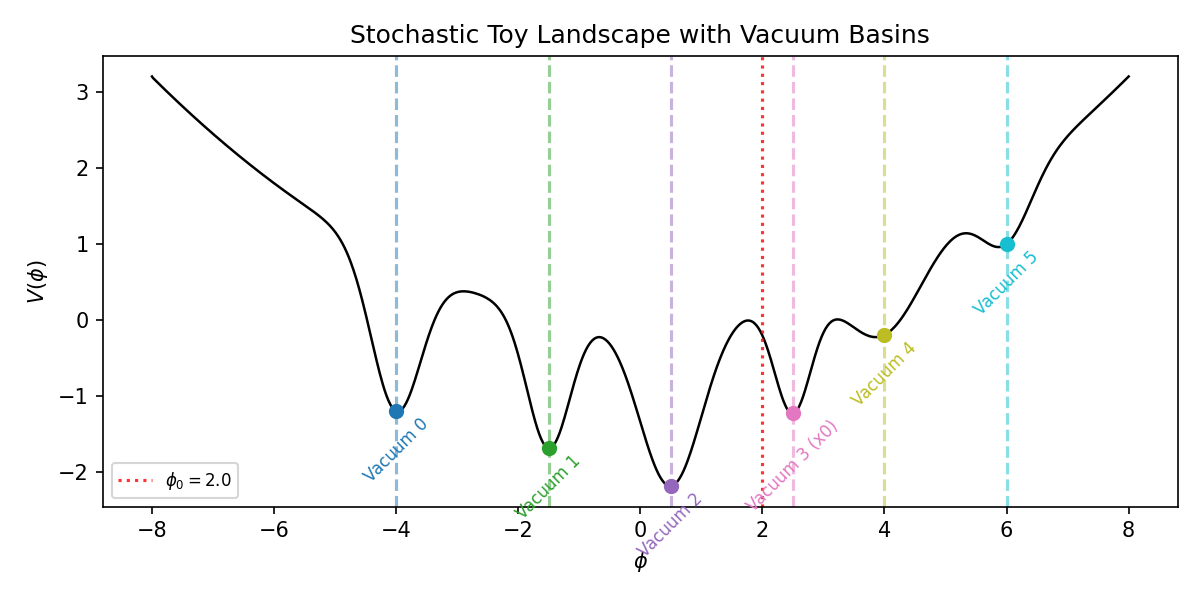
\includegraphics[width=\columnwidth]{figures/fig_01_landscape_basins.png}
  \caption{Stochastic toy landscape $V(\phi)$ with six vacuum basins.
  The observable patch $\phi_0 = 2.0$ (red dotted line) lies in basin~3.
  Each basin is assigned an effective physics vector $\boldsymbol{\theta}$.}
  \label{fig:landscape}
\end{figure}

\subsection{Basin assignment}

Each well center defines a vacuum basin.
Basin identity is determined by the nearest local minimum of the potential.
The observable patch at $\phi_0 = 2.0$ is identified with basin~3 via
\verb|landscape.identify_basin(phi0)|, not from the first sampled trajectory.
This matters for the stress test, where the first trajectory can land in any basin.

\subsection{Initial conditions and dynamics}

Initial field values are sampled from a normal distribution
$\phi_{\rm init} \sim \mathcal{N}(\phi_0, \sigma^2)$ with $\sigma = 1.5$
by default.
Each trajectory evolves via a Langevin-like stochastic differential equation
over 80~$e$-folds with time step $\Delta t = 0.1$.
The main run uses $N = 10,\!000$ trajectories; stress tests use $N = 2,\!000$.

\subsection{Effective physics vector}

Each basin $v$ is assigned a physics vector
$\boldsymbol{\theta}(v) = (\Lambda_{\rm eff}, G_{\rm eff}, Q_{\rm fluct}, T_{\rm reh})$
with toy values reflecting different phenomenological profiles.
These values are arbitrary placeholders; they demonstrate the mechanism
of unobserved-sector reweighting but carry no claim about real cosmology.

\subsection{Cutoff list}

We evaluate measures at cutoffs
$N_k \in \{100, 250, 500, 1000, 2500, 5000, 10000\}$.
Cutoffs exceeding the total number of sectors are dropped.

% Experiments
\section{Experiments and diagnostics}
\label{sec:experiments}

We run twelve experiments to test \ISR against the global census baseline.
Table~\ref{tab:kernel_roles} summarizes kernel roles.

\begin{table}[t]
  \centering
  \caption{Kernel roles, evidence status, and rationale. Evidence kernels are used in main ISR results; diagnostic kernels illustrate sensitivity to design choices.}
  \label{tab:kernel_roles}
  \begin{tabular}{lllp{5cm}}
    \toprule
    Kernel & Role & Evidence & Reason \\
    \midrule
    Gaussian & Primary locality kernel & Evidence & Exponential decay in field-space distance; standard smoothing kernel. \\
    Exponential & Robustness kernel & Evidence & Heavier tail than Gaussian; tests sensitivity to kernel shape. \\
    \texttt{same\_basin} & Diagnostic & Diagnostic & Trivially conditions on $x_0$ basin membership; no field-distance resolution. \\
    \texttt{ancestry\_proxy} & Diagnostic & Diagnostic & Uses trajectory index as a proxy for branch ancestry; not a true causal ancestry graph. \\
    \bottomrule
  \end{tabular}
\end{table}


\subsection{Experiment 1: Global census baseline}
\label{exp:1}

Compute $P_{\rm global}(v)$ at each cutoff $N_k$.
\emph{Purpose}: quantify cutoff dependence of naive counting.
\emph{Expected failure}: distribution shifts toward the largest basin as $N$ increases.

The global census is the natural null hypothesis: it treats all generated sectors
as equally relevant regardless of their field-space location.
A measure must justify why some sectors count more than others, and \ISR provides
a specific locality-based answer.
The global census is therefore the correct baseline---not because it is expected
to work well (it is not), but because it represents the simplest possible measure
that makes no distinction between sectors.
If \ISR does not improve upon it, the locality proposal adds no value.

\subsection{Experiment 2: ISR locality-weighted measure}
\label{exp:2}

Compute $P_{\rm ISR}(v \mid x_0)$ using a Gaussian kernel ($\ell = 1$)
with field-space distance.
\emph{Purpose}: test whether locality weighting shifts probability toward the
$x_0$ basin and improves stability.

\subsection{Experiment 3: Cutoff stability}
\label{exp:3}

Compare $D_{\rm KL}$ and Wasserstein distances across all cutoffs
for both measures, and for multiple kernels.
\emph{Purpose}: identify which kernel---measure combinations converge.

\subsection{Experiment 4: Kernel sensitivity}
\label{exp:4}

Vary $\ell$ and kernel functional form to check sensitivity.
\emph{Purpose}: ensure results are not an artifact of one kernel choice.

\subsection{Experiment 5: Basin-boundary diagnostics}
\label{exp:5}

At fixed distance thresholds, compute the fraction of ``nearby'' sectors
($d < d_{\rm thr}$) that lie in a different basin from $x_0$.
\emph{Purpose}: measure how often the locality assumption fails.

\subsection{Experiment 6: Configuration-space locality diagnostics}
\label{exp:6}

For three distance metrics (field-space, initial-field, basin-transition),
evaluate continuity score, basin-exception rate, and locality-failure rate.
\emph{Purpose}: characterize the structure of locality violations.

\subsection{Experiment 7: Kernel-weighted sector averaging}
\label{exp:7}

Compute $c_{\rm eff}(\ell)$ at varying $\ell$ to show unobserved-sector mixing.
\emph{Purpose}: illustrate kernel-weighted sector averaging.

\subsection{Experiment 8: Stress test}
\label{exp:8}

Repeat experiments~1 and~2 for $\sigma \in \{0.5, 1.0, 1.5, 2.0, 3.0\}$ with
seeds $1$ through $20$ ($100$ total runs), $N = 2,\!000$ per run.
\emph{Purpose}: test robustness across random and systematic variation.

\subsection{Experiment 9: Ell sensitivity scan}
\label{exp:9}

Vary $\ell$ across 15 values in logspace from 0.05 to 10.0 with Gaussian and
exponential kernels.
For each $\ell$, record final KL drift, effective sample size $N_{\rm eff}$,
basin exception rate, effective coefficient $\Lambda_{\rm eff}$, and
convergence rate.
The convergence rate is defined as the slope of log KL drift versus log cutoff,
$d(\log{\rm KL}) / d(\log N)$, estimated by linear regression over the
log--log curve.
A convergence rate of $-1$ indicates ${\rm KL} \propto 1/N$, matching the
parametric rate of a well-behaved Monte Carlo estimator; rates approaching $0$
indicate that additional samples do not improve the estimate.
Also run a randomized-distance null control (shuffled sector--distance
pairings) to verify that the improvement is not an artifact of the kernel
smoothing.
\emph{Purpose}: map the sweet spot of $\ell$ where ISR provides meaningful
improvement without being trivially narrow or approaching global census.

\subsection{Experiment 10: Sigma--ell boundary}
\label{exp:10}

Grid over $\sigma \in \{0.5, 1.0, 1.5, 2.0, 3.0\}$ and
$\ell \in \{0.1, 0.25, 0.5, 1.0, 2.0\}$, 5 seeds per cell
($125$ total runs), $N = 2,\!000$ per run.
\emph{Purpose}: identify any $(\sigma, \ell)$ region where ISR underperforms
the global census.

\subsection{Experiment 11: Flat-parent composition sanity check}
\label{exp:11}

For each cutoff, compose the \ISR weighting with a flat parent measure
(equal weight to all sectors). The composition applies \ISR re-weighting
on top of the parent baseline and checks that the resulting
cutoff-stability trend is consistent with the standalone \ISR result.
\emph{Purpose}: sanity check that \ISR can be stacked with a trivial
parent measure without introducing numerical inconsistencies.

\subsection{Experiment 12: Landscape perturbation robustness}
\label{exp:12}

Shift all well centers $\mu \to \mu + 0.5$ in the toy landscape and repeat
Experiments~1 and~2 at $\sigma \in \{1.5, 3.0\}$, 5 seeds per cell.
The perturbed landscape preserves the same number of basins and the same 
basin physics vectors $\boldsymbol{\theta}$, but shifts basin boundaries
relative to $\phi_0$.
\emph{Purpose}: verify that \ISR improvement is not an artifact of the
specific well placement in the unperturbed landscape.

% Results
\section{Results}
\label{sec:results}

We organize results around eight claims.

\subsection{Claim 1: ISR changes the selected basin}

Table~\ref{tab:main_distribution} shows the final probability distributions at
$N = 10,\!000$. The global census favors vacuum~2 by raw count, while
\ISR (Gaussian $\ell = 1$) shifts weight toward vacuum~3, the basin
containing $x_0$.

\begin{table}[t]
  \centering
  \caption{Probability distribution over vacuum basins at final cutoff $N=10000$. ISR uses a Gaussian kernel with $\ell=1$. Metrics: KL drift $=3.58\times10^{-4}$ (global) vs $1.27\times10^{-4}$ (ISR); Wasserstein $=9.30\times10^{-3}$ vs $6.41\times10^{-3}$; both measures are stable under cutoff extension.}
  \label{tab:main_distribution}
  \begin{tabular}{lccc}
    \toprule
    Vacuum & Global census & ISR Gaussian $\ell=1$ & Difference \\
    \midrule
    0 & 0.000700 & 0.000000 & -0.000700 \\
    1 & 0.044000 & 0.000207 & -0.043793 \\
    2 & 0.396000 & 0.264742 & -0.131258 \\
    3 & 0.358600 & 0.661812 & +0.303212 \\
    4 & 0.186600 & 0.073217 & -0.113383 \\
    5 & 0.014100 & 0.000023 & -0.014077 \\
    \bottomrule
  \end{tabular}
\end{table}


Fig.~\ref{fig:global_vs_isr} visualizes this shift.
The global census allocates 39.6\% to vacuum~2 and 35.9\% to vacuum~3.
\ISR reverses this: vacuum~2 falls to 26.5\% while vacuum~3 rises to 66.2\%.

\begin{figure}[t]
  \centering
  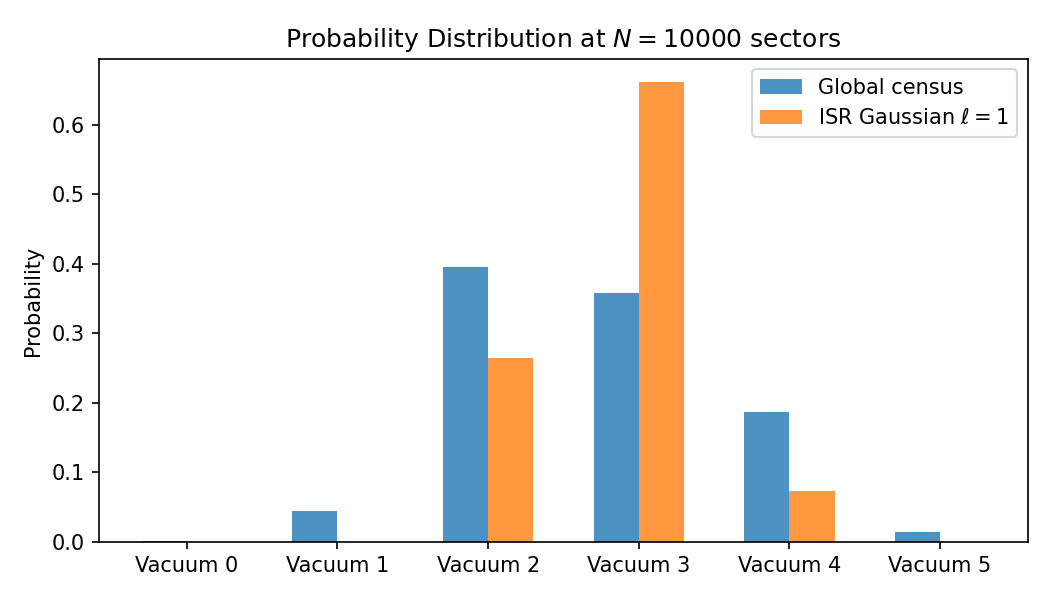
\includegraphics[width=\columnwidth]{figures/fig_02_global_vs_isr_distribution.png}
  \caption{Probability distribution at $N = 10,\!000$ sectors.
  \ISR shifts weight from the most populous vacuum~2 to the local vacuum~3.}
  \label{fig:global_vs_isr}
\end{figure}

\subsection{Claim 2: ISR improves finite-sample cutoff stability}

Table~\ref{tab:main_distribution} shows that \ISR reduces the final KL drift
from $3.58\times10^{-4}$ (global census) to $1.27\times10^{-4}$ (ISR),
an improvement by approximately a factor of two.
The Wasserstein distance improves from $9.30\times10^{-3}$ to $6.41\times10^{-3}$.
Fig.~\ref{fig:kl_drift} compares the two measures.

\begin{figure}[t]
  \centering
  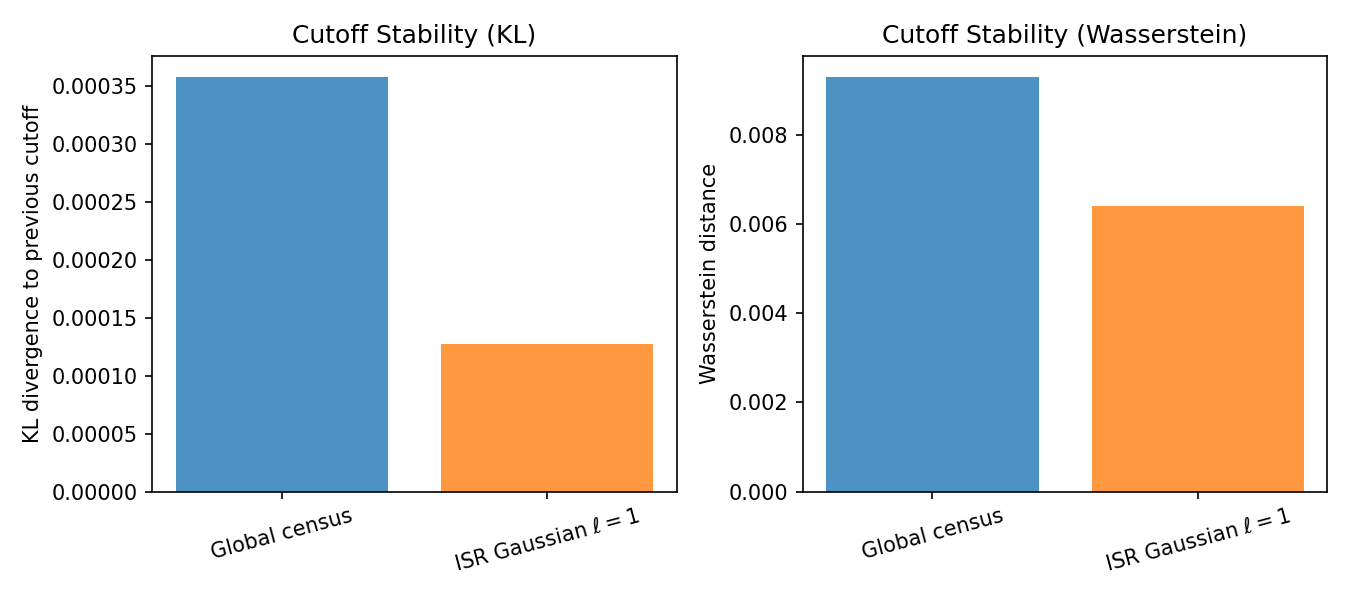
\includegraphics[width=\columnwidth]{figures/fig_03_kl_drift_global_vs_isr.png}
  \caption{KL divergence and Wasserstein distance for global census and
  \ISR (Gaussian $\ell = 1$) at $N = 10,\!000$.
  \ISR reduces both metrics.}
  \label{fig:kl_drift}
\end{figure}

\subsection{Claim 3: ISR is robust across stress tests}

Table~\ref{tab:stress_summary} summarizes the 100-run stress test.
\ISR improves over global census in 98 of 100 runs.
The improvement ratio is largest at intermediate $\sigma$ values
($1.0$--$2.0$), where the initial-condition spread samples multiple basins
but remains concentrated enough for locality weighting to be effective.

\begin{table}[t]
  \centering
  \caption{Stress test summary by $\sigma$. Each row aggregates 20 random seeds with $N=2000$ trajectories per run.}
  \label{tab:stress_summary}
  \begin{tabular}{lcccccc}
    \toprule
    $\sigma$ & Global mean KL & ISR mean KL & Median improv. & ISR wins / total & Mean $n_{\rm vacua}$ \\
    \midrule
    0.5 & 0.0008 & 0.0003 & 2.1$\times$ & 20/20 & 3.0 \\
    1.0 & 0.0013 & 0.0003 & 3.9$\times$ & 20/20 & 4.7 \\
    1.5 & 0.0012 & 0.0003 & 4.7$\times$ & 20/20 & 6.0 \\
    2.0 & 0.0011 & 0.0003 & 3.7$\times$ & 20/20 & 6.0 \\
    3.0 & 0.0010 & 0.0004 & 3.4$\times$ & 18/20 & 6.0 \\
    \bottomrule
  \end{tabular}
\end{table}


Fig.~\ref{fig:stress_improvement} shows the distribution of improvement ratios
by $\sigma$.

\begin{figure}[t]
  \centering
  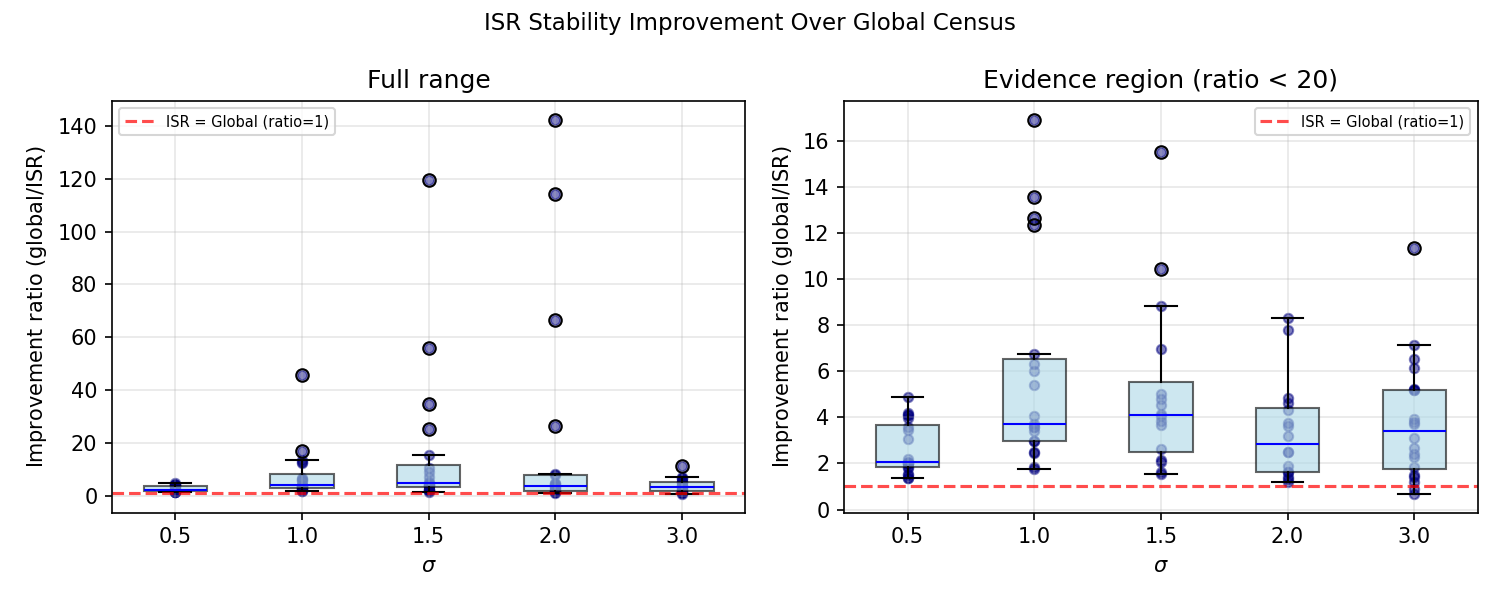
\includegraphics[width=\columnwidth]{figures/fig_07_stress_improvement_by_sigma.png}
  \caption{Improvement ratio $D_{\rm KL}^{\rm global} / D_{\rm KL}^{\rm ISR}$
  by $\sigma$. Points above 1 (dashed red line) indicate \ISR outperforms
  global. Boxes show quartiles across 20 seeds per $\sigma$.}
  \label{fig:stress_improvement}
\end{figure}

\subsection{Claim 4: Locality has basin-boundary exceptions}

The configuration-space locality diagnostics (Fig.~\ref{fig:basin_exception})
reveal that locality is not uniformly respected.
Using initial-field distance, the basin-exception rate rises from 5\% at
threshold 0.1 to 52\% at threshold 2.0 (Fig.~\ref{fig:basin_exception}).
This means that as we widen the ``nearby'' definition, more sectors that are
close in initial field value lie in different vacuum basins.

\begin{figure}[t]
  \centering
  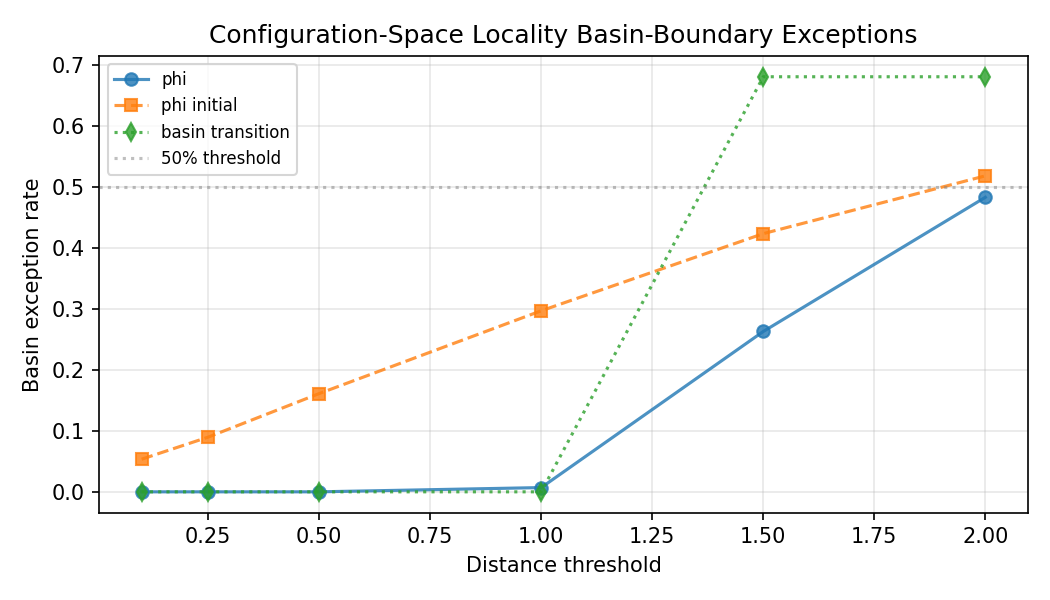
\includegraphics[width=\columnwidth]{figures/fig_05_basin_exception_rate.png}
  \caption{Basin-exception rate vs. distance threshold for three distance
  metrics. The initial-field metric (dashed) shows the most gradual rise,
  making it the most relevant diagnostic for locality continuity.}
  \label{fig:basin_exception}
\end{figure}

The continuity score (fraction of near same-basin pairs with small $\theta$
difference) is 1.0 for all thresholds: when sectors are in the same basin,
their effective physics is identical by construction.
Locality failures (near same-basin pairs with different $\theta$) are zero
for the same reason.
The relevant failure mode is the basin exception---nearby sectors in
different basins---which is captured by our diagnostics.

\subsection{Claim 5: Kernel-weighted sector averaging}

The kernel-weighted sector averaging (Table~\ref{tab:effective_coefficients}
in Appendix~\ref{app:supplementary}) shows aggregate coefficients as a
function of $\ell$.
At $\ell = 0.1$, the aggregate $\Lambda_{\rm eff} = 2.0$,
reflecting near-pure $x_0$ basin.
At $\ell = 2.0$, $\Lambda_{\rm eff} = 1.44$, shifted by mixing with
unobserved-sector vacua.
This averaging is a numerical consequence of the assigned physics vectors
$\boldsymbol{\theta}(v)$ and the kernel weighting; it is illustrative
of how sector weighting changes aggregate toy parameters in a
controlled toy setting, not a derivation of physical running couplings.

\subsection{Claim 6: Ell sensitivity reveals a sweet spot}

\begin{figure}[htbp]
  \centering
  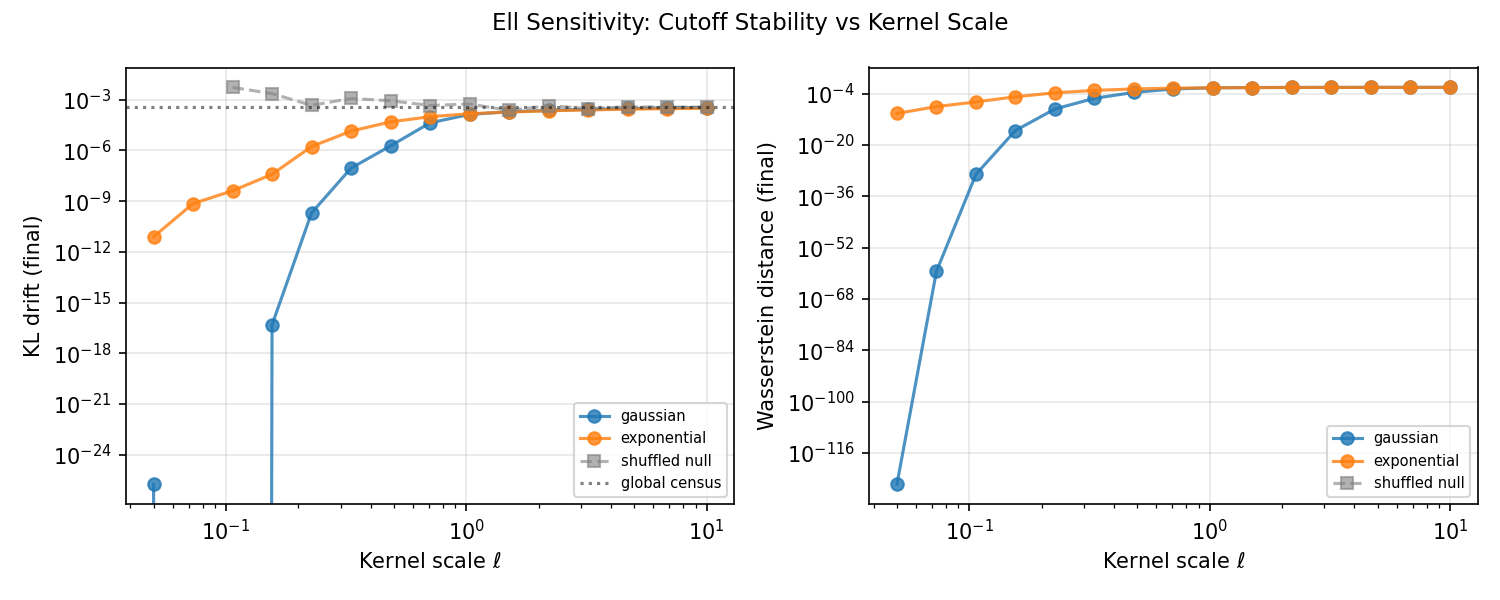
\includegraphics[width=\columnwidth]{figures/fig_11_ell_sensitivity_kl.png}
  \caption{KL drift and Wasserstein distance vs.\ kernel scale $\ell$.
  The black dotted line is the global-census baseline; the gray dashed
  line is the shuffled null control.}
  \label{fig:ell_sensitivity_kl}
\end{figure}

Fig.~\ref{fig:ell_sensitivity_kl} shows the evolution of ISR stability
metrics across $\ell$ (see Table~\ref{tab:ell_sensitivity} in
Appendix~\ref{app:supplementary} for the full data).
We define $N_{\rm eff} = (\sum_i w_i)^2 / \sum_i w_i^2$,
where $w_i = K_\ell[d(x_i, x_0)]$; $N_{\rm eff} \approx N$ when the kernel
weights all sectors equally and $N_{\rm eff} \ll N$ when only a few sectors
dominate.
Three regimes emerge:

\begin{itemize}
  \item \textbf{Narrow kernel} ($\ell \lesssim 0.2$): $N_{\rm eff} \ll N$,
        KL drift is vanishingly small (below $10^{-25}$ for $\ell=0.05$).
        This is an artifact: the kernel isolates only the
        $x_0$ basin and the ISR distribution is nearly a delta function.
        Reported KL divergences in this regime are not meaningful indicators
        of physical stability (see Appendix~\ref{app:degenerate}).
  \item \textbf{Sweet spot} ($0.5 \lesssim \ell \lesssim 1.5$):
        $N_{\rm eff} \approx 0.3$--$0.9\,N$, KL drift is $2$--$3\times$
        below global census, and basin exceptions remain below 30\%.
        The convergence rate $d(\log{\rm KL})/d(\log N) \approx -1.0$,
        comparable to global census.
  \item \textbf{Broad kernel} ($\ell \gtrsim 3$): $N_{\rm eff} \approx N$,
        KL drift approaches the global census value, and basin exceptions
        saturate above 60\%. ISR reduces to global weighting.
\end{itemize}

The randomized-distance null control (shuffled sector--distance pairings)
produces KL drift that always exceeds the correctly paired ISR at the same
$\ell$ and is typically comparable to or larger than the global-census
baseline.
This shows that the improvement is not a generic artifact of kernel smoothing;
it depends on preserving the field-space distance structure encoded by the
toy landscape.

\subsection{Claim 7: ISR remains favorable in the non-degenerate sigma--ell region}

\begin{table}[htbp]
  \centering
  \caption{Sigma-by-ell boundary: mean improvement ratio (global KL / ISR KL)
  across 5 seeds per cell, non-degenerate regime ($\ell \ge 0.50$).
  The degenerate small-$\ell$ columns ($\ell=0.10, 0.25$) are reported in
  Appendix~\ref{app:degenerate}.}
  \label{tab:sigma_ell_boundary}
  \small
  \begin{tabular}{lccc}
    \toprule
    $\sigma \backslash \ell$ & 0.50 & 1.00 & 2.00 \\
    \midrule
    0.5 & 68.5 & 3.12 & 1.28 \\
    1.0 & 142.5 & 5.97 & 1.86 \\
    1.5 & 240.0 & 5.38 & 2.35 \\
    2.0 & 103.1 & 7.68 & 4.40 \\
    3.0 & 58.5 & 6.27 & 2.46 \\
    \bottomrule
  \end{tabular}
\end{table}


\begin{figure}[htbp]
  \centering
  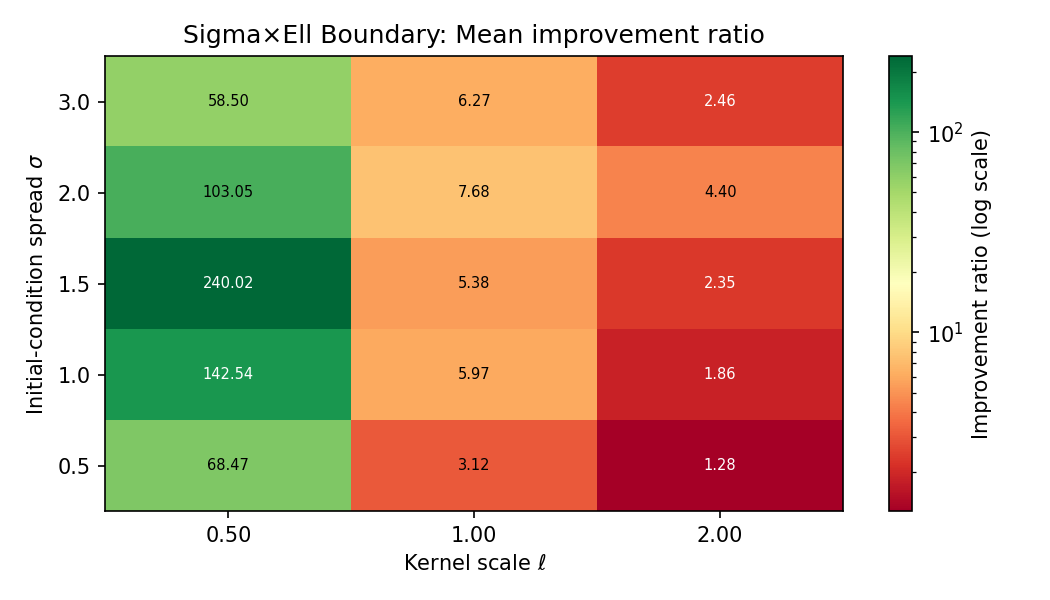
\includegraphics[width=\columnwidth]{figures/fig_13_sigma_ell_mean_improvement.png}
  \caption{Mean improvement ratio (global KL / ISR KL) across the sigma--ell
  grid. All non-degenerate cells ($\ell \ge 0.50$) exceed 1.}
  \label{fig:sigma_ell_boundary}
\end{figure}

The sigma--ell boundary experiment (Experiment~\ref{exp:10}) is a separate
scan from the 100-run stress test (Experiment~\ref{exp:8}).
Table~\ref{tab:sigma_ell_boundary} summarizes the non-degenerate region
($\ell \ge 0.50$) of the sigma--ell grid
(5 sigma values $\times$ 3 ell values $\times$ 5 seeds).
The improvement ratio remains $1.3$--$270$, with no failure case (ISR
underperforming global census) across any tested sigma--ell cell.
ISR improves over global census in \emph{every} tested non-degenerate cell of
the grid (improvement ratio $>1$).
The improvement is strongest at large $\sigma$ (broad initial-condition spreads),
where the global census is most cutoff-dependent.
Degenerate small-$\ell$ results ($\ell=0.10, 0.25$) are reported in
Appendix~\ref{app:degenerate}.

\subsection{Claim 8: ISR improvement is robust to landscape perturbation}

The landscape perturbation test (Experiment~\ref{exp:12}) shifts all well
centers by $+0.5$ while preserving the number of basins and physics vectors.
Table~\ref{tab:landscape_perturbation} shows the mean improvement ratio across
5 seeds.
In this limited perturbation test, ISR improves over global census in all
tested runs (all ratios $>1$), with qualitatively similar performance to
the unperturbed landscape.
The perturbation suggests that ISR improvement is not solely an artifact of
the original well placement.

\begin{table*}[t]
  \centering
  \caption{Landscape perturbation robustness: mean improvement ratio (global KL / ISR KL) for shifted well positions ($\mu \to \mu + 0.5$), 5 seeds per cell. ISR improves over global census in all tested runs (all ratios $>1$).}
  \label{tab:landscape_perturbation}
  \small
  \begin{tabular}{lccc}
    \toprule
    Landscape & $\sigma$ & Mean improvement ratio & Range \\
    \midrule
    Original & 1.5 & 11.3 & 2.0--32.9 \\
    Perturbed & 1.5 & 6.2 & 2.2--13.1 \\
    Perturbed & 3.0 & 7.0 & 1.9--20.6 \\
    \bottomrule
  \end{tabular}
\end{table*}


% Discussion
\section{Discussion}
\label{sec:discussion}

Locality weighting changes the measure by suppressing the contribution of
sectors far from the observable patch in field space.
This differs from global counting, where the most populous basin dominates
regardless of locality.

Cutoff stability matters because a measure with uncontrolled cutoff dependence
does not produce well-defined predictions.
The improvement of \ISR over global census is numerical and empirical, not a
theorem, but it demonstrates that locality weighting is a viable direction
for measure construction.

Basin boundaries limit locality continuity.
As the initial-condition spread $\sigma$ increases, more trajectories land in
distant basins, diluting the locality signal.
This is physical---there is no locality principle that guarantees nearby
field values share the same vacuum---and it motivates the diagnostics we
introduce.

The kernel-weighted sector averaging (Sec.~\ref{sec:results}) loosely echoes
the bookkeeping role of coarse-graining in effective field theory, but no
physical running-coupling interpretation is implied.

Several directions for future work are natural:
\begin{itemize}
  \item Replacing the ancestry proxy with a true causal ancestry graph
        based on branching history.
  \item Extending to multi-field landscapes with more realistic potentials.
  \item Incorporating Coleman--De Luccia transition rates between basins.
  \item Adding explicit decoherence or an open-system treatment of the
        environment.
  \item Bayesian model comparison against other measure proposals using
        synthetic observations.
  \item Analytic investigation of convergence conditions for different
        kernel families.
\end{itemize}

% Limitations
\section{Limitations}
\label{sec:limitations}

This work is a numerical toy demonstration with specific limitations:

\begin{itemize}
  \item \textbf{Toy landscape.} The potential is one-dimensional with six
        wells. Realistic inflationary landscapes involve many fields and
        complex tunneling dynamics.
  \item \textbf{Assigned physics.} Vacuum physics vectors
        $\boldsymbol{\theta}(v)$ are assigned, not derived from quantum
        gravity or even from the potential shape.
  \item \textbf{Simplified $\theta$ vectors.} Each basin has exactly one
        physics vector; there is no intra-basin variation.
  \item \textbf{Ancestry proxy.} The \texttt{ancestry\_proxy} kernel uses
        trajectory index as a proxy for causal ancestry. This is not true
        branch ancestry and should be treated as diagnostic only.
  \item \textbf{Diagnostic-only kernels.} \texttt{same\_basin} is
        diagnostic-only because it trivially conditions on $x_0$ basin
        membership.
  \item \textbf{Kernel and $\ell$ dependence.} Results depend on the choice
        of kernel and scale parameter $\ell$. We report sensitivity
        (Experiment~\ref{exp:4}) but do not provide a first-principles derivation
        of the optimal kernel.
  \item \textbf{Numerical, not analytic.} The observed stability improvement
        is an empirical property of this simulation, not a proven theorem
        about locality-weighted measures.
  \item \textbf{No physical claim about multiverse reality.} This simulation
        does not establish the existence or detectability of pocket universes.
  \item \textbf{Configuration-space locality as a modeling prior.} The locality
        assumption (sectors near $x_0$ in field space are more relevant) is a
        modeling prior, not an observable causal relation. It is justified only
        inside a shared-landscape model.
\end{itemize}

\ISR should be judged by stability, robustness, and failure transparency,
not by whether it can be tuned to prefer a desired vacuum.

% Conclusion
\section{Conclusion}
\label{sec:conclusion}

We proposed \isr (\ISR), a configuration-space locality-weighted sector framework for
regulating toy eternal-inflation ensembles.
In a stochastic landscape simulation with 10,000 trajectories and six
vacuum basins, \ISR shifts probability mass toward the basin local to the
observable patch and improves trajectory-cutoff stability relative to a naive
global census by approximately a factor of two in KL divergence.
Across 100 sigma-by-seed stress tests, \ISR outperforms global census in
98 cases.
A shifted-well landscape perturbation suggests that the improvement is not
solely an artifact of the original well placement.

An ell-sensitivity scan (15 values from 0.05 to 10.0) reveals a sweet spot at
$\ell \approx 0.5$--$1.5$ where $N_{\rm eff}$ is large enough for statistical
power and basin-exception rates remain below 30\%.
A randomized-distance null control shows that the improvement is not a generic
artifact of kernel smoothing; it depends on preserving the field-space distance
structure encoded by the toy landscape.
In the non-degenerate region of the sigma-by-ell grid, ISR improves over global
census across every tested cell. Degenerate small-ell cells are excluded from
this evidence claim and reported separately in Appendix~\ref{app:degenerate}.

These results do not solve the eternal-inflation measure problem.
They demonstrate a reproducible toy framework for testing locality-weighted
measures, with built-in diagnostics that expose when and why the weighting
succeeds or fails.
The code, data, and paper source are available at
\url{https://github.com/jenholm/physics_models/tree/main/inflationary-sector-renormalization}.


\bibliographystyle{apsrev4-2}
\bibliography{bib/references}

\newpage
\appendix
% Appendix A: Simulation details
\section{Simulation details}
\label{app:simulation}

\subsection{Configuration}

The simulation is configured via YAML files in \texttt{configs/}:
\begin{itemize}
  \item \texttt{base.yaml}: simulation parameters, kernel choices, cutoffs,
        initial conditions.
  \item \texttt{landscapes.yaml}: well positions $(\mu, V_0)$, basin physics
        vectors $\boldsymbol{\theta}$.
  \item \texttt{kernels.yaml}: kernel names, $\ell$ values, distance types.
\end{itemize}

\subsection{Numerical parameters}

\begin{itemize}
  \item $n_{\rm trajectories} = 10,\!000$ (main run).
  \item Stress test: $100$ runs ($5 \times \sigma \times 20$ seeds),
        $n_{\rm trajectories} = 2,\!000$ per run.
  \item $\sigma_{\rm initial} = 0.5, 1.0, 1.5, 2.0, 3.0$.
  \item Seeds: $1$--$20$.
  \item Observable $\phi_0 = 2.0$.
  \item Primary kernel: Gaussian $\ell = 1.0$.
  \item $e$-folds: $80$, time step $\Delta t = 0.1$.
\end{itemize}

\subsection{Measure computation}

The global census and \ISR measures are computed at each cutoff $N_k$.
KL divergence uses the union of support labels (vacua appearing in either
distribution), with zero probability treated as $10^{-12}$ for
logarithmic stability.
The 1-Wasserstein distance is computed over the cumulative distribution
function of vacuum probabilities.

\subsection{Kernel-weighted sector averaging}

For each $\ell \in \{0.1, 0.25, 0.5, 1.0, 2.0\}$, the aggregate effective
coefficient $c_{\rm eff}(\ell)$ is computed at the final cutoff using
Eq.~\eqref{eq:effective_flow}.
Per-vacuum coefficients are also reported in the output data.

% Appendix B: Failure cases
\section{Failure cases}
\label{app:failures}

Table~\ref{tab:failure_cases} lists the two stress-test runs where
\ISR underperforms global census.
Both occur at $\sigma = 3.0$, the broadest initial-condition spread.

\begin{table}[t]
  \centering
  \caption{Failure cases: ISR underperforms global census. Both cases occur at $\sigma=3.0$, the broadest initial-condition spread.}
  \label{tab:failure_cases}
  \begin{tabular}{lccccc}
    \toprule
    $\sigma$ & Seed & ISR KL & Global KL & Ratio & Possible cause \\
    \midrule
    3.0 & 13 & 0.0007 & 0.0005 & 0.68 & Broad initial spread samples vacua far from $x_0$; kernel overlap is thin. \\
    3.0 & 14 & 0.0012 & 0.0010 & 0.89 & Broad initial spread samples vacua far from $x_0$; kernel overlap is thin. \\
    \bottomrule
  \end{tabular}
\end{table}


In these runs, the broad initial spread causes many trajectories to sample
vacua far from $x_0$, reducing the effective sample of local sectors.
The Gaussian kernel assigns low weight to distant sectors, and the resulting
measure fluctuates more than the global census, which includes all sectors
regardless of distance.

Fig.~\ref{fig:failure_cases} shows the full $\sigma = 3.0$ distribution
of KL values by seed.

\begin{figure}[t]
  \centering
  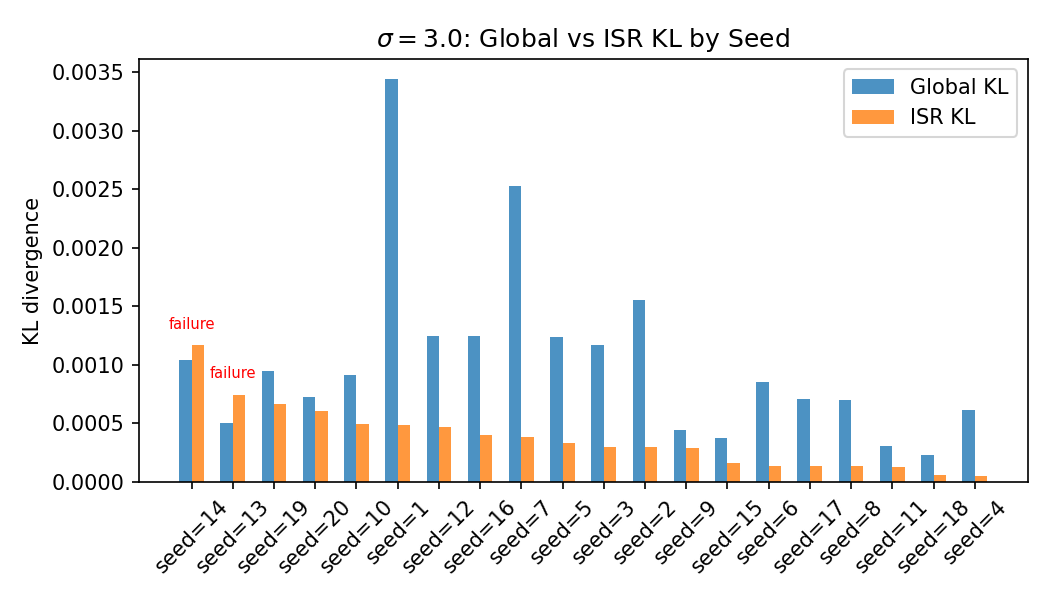
\includegraphics[width=\columnwidth]{figures/fig_08_failure_cases_sigma3.png}
  \caption{KL divergence at $\sigma = 3.0$ for global census and \ISR
  by seed. Two seeds (13 and 14) show \ISR above global.}
  \label{fig:failure_cases}
\end{figure}

\subsection{Diagnostics for both failure cases}

Table~\ref{tab:failure_diagnostics} shows diagnostic metrics for both failure
seeds alongside the non-failure mean at $\sigma=3.0$.
The diagnostics are similar across all three columns: both failure seeds have
$N_{\rm eff}/N$ near 0.48--0.49 and weighted mass in the $x_0$ basin in the
55--59\% range, comparable to the non-failure mean.
The failures are not driven by dramatically different diagnostics but by
borderline cases where the ISR KL divergence slightly exceeds the global
census value by a small margin.

\begin{table*}[t]
  \centering
  \caption{Diagnostic metrics for failure seeds 13 and 14
  ($\sigma=3.0$, $\ell=1.0$, Gaussian kernel) compared with non-failure mean
  at $\sigma=3.0$.}
  \label{tab:failure_diagnostics}
  \small
  \begin{tabular}{lccc}
    \toprule
    Metric & Seed 13 & Seed 14 & Non-failure mean \\
    \midrule
    Effective sample size $N_{\rm eff}$ & 977 & 960 & 963 \\
    $N_{\rm eff} / N$ & 0.49 & 0.48 & 0.48 \\
    Weighted mass in $x_0$ basin & 58.8\% & 54.7\% & 57.7\% \\
    Vacuum distribution entropy & 0.94 nats & 0.97 nats & 0.95 nats \\
    Top vacuum probability & 58.8\% & 54.7\% & 57.7\% \\
    Basin exception rate ($d < \ell$) & 0.0\% & 0.0\% & 0.0\% \\
    Weight concentration $\max(w) / \sum w$ & $1.58\times10^{-3}$ & $1.63\times10^{-3}$ & $1.58\times10^{-3}$ \\
    \bottomrule
  \end{tabular}
\end{table*}

These failures are informative: they show that locality weighting is not
universally beneficial and that broad initial-condition spreads can dilute
the signal. Reporting them honestly strengthens rather than weakens the
analysis.

% Appendix C: Reproducibility
\section{Code and reproducibility}
\label{app:reproducibility}

The full codebase is available at
\url{https://github.com/jenholm/physics_models/tree/main/inflationary-sector-renormalization}.
All results in this paper were produced with the following software versions:

\begin{itemize}
  \item Commit \texttt{fb1b497} of this repository.
  \item Python 3.12.3 with: numpy 2.4.6, scipy 1.17.1, pandas 3.0.3,
        matplotlib 3.10.9, PyYAML 6.0.1.
  \item Config hashes: base.yaml \texttt{1fcc4c5c9ac7},
        landscapes.yaml \texttt{ef664ae36835}.
  \item A working \LaTeX\ distribution with revtex4-2, bibtex and
        standard packages.
\end{itemize}

\subsection{Running experiments}

\begin{verbatim}
git clone https://github.com/jenholm/physics_models.git
cd physics_models/inflationary-sector-renormalization
python -m venv .venv
source .venv/bin/activate
pip install -r requirements.txt
python -m compileall isr experiments
python run_all.py
\end{verbatim}

\subsection{Expected outputs}

The script \texttt{run\_all.py} runs all twelve experiments sequentially.
Key output files include:

\begin{itemize}
  \item \texttt{outputs/isr\_result\_summary.md} --- compiled Markdown report.
  \item \texttt{outputs/global\_measure\_vs\_cutoff.json} --- global census
        probabilities per cutoff.
  \item \texttt{outputs/isr\_measure\_vs\_cutoff.json} --- \ISR probabilities.
  \item \texttt{outputs/kernel\_comparison\_table.csv} --- cutoff stability
        by kernel.
  \item \texttt{outputs/stress\_test\_results.csv} --- all 100 stress-test runs.
  \item \texttt{outputs/stress\_test\_summary.json} --- aggregated stress metrics.
  \item \texttt{outputs/configuration\_space\_locality\_summary.csv} ---
        configuration-space locality diagnostics.
  \item \texttt{outputs/kernel\_weighted\_sector\_averaging.csv} ---
        kernel-weighted sector averaging.
  \item \texttt{outputs/ell\_sensitivity\_results.csv} --- ell scan (Exp~9).
  \item \texttt{outputs/ell\_sensitivity\_summary.json} --- aggregated ell metrics.
  \item \texttt{outputs/sigma\_ell\_boundary\_results.csv} --- sigma-by-ell grid (Exp~10).
  \item \texttt{outputs/sigma\_ell\_boundary\_summary.json} --- aggregated boundary metrics.
  \item \texttt{outputs/flat\_parent\_composition.json} --- composed-measure sanity check (Exp~11).
  \item \texttt{outputs/landscape\_perturbation\_results.json} --- perturbed-landscape robustness (Exp~12).
\end{itemize}

\subsection{Paper figures and tables}

Figures are generated by \texttt{paper/generate\_figures.py}.
Tables are generated by \texttt{paper/generate\_tables.py}.
The paper is built with \texttt{make} in the \texttt{paper/} directory.

% Appendix D: Supplementary tables and figures
\section{Supplementary material}
\label{app:supplementary}

\subsection{Kernel-weighted sector averaging}
\label{app:coeff_averaging}

\begin{table}[t]
  \centering
  \caption{Kernel-weighted sector averaging across kernel scale $\ell$ at final cutoff $N=10000$. As $\ell$ increases, unobserved-sector mixing shifts aggregate toy coefficients away from the pure $x_0$ basin values.}
  \label{tab:effective_coefficients}
  \begin{tabular}{lccccc}
    \toprule
    $\ell$ & Lambda\_Eff & G\_Eff & Q\_Fluctuation & Reheating\_Temp & Interpretation \\
    \midrule
    0.1 & 2.0000 & 0.7000 & 0.1000 & 200.0000 & Near-pure $x_0$ basin \\
    0.25 & 2.0000 & 0.7000 & 0.1000 & 200.0000 & Near-pure $x_0$ basin \\
    0.5 & 1.9817 & 0.7089 & 0.1072 & 198.1747 & Moderate mixing \\
    1.0 & 1.6781 & 0.8499 & 0.2381 & 167.8119 & Strong unobserved-sector mixing \\
    2.0 & 1.4432 & 0.9497 & 0.3497 & 144.2906 & Strong unobserved-sector mixing \\
    \bottomrule
  \end{tabular}
\end{table}


\begin{figure}[t]
  \centering
  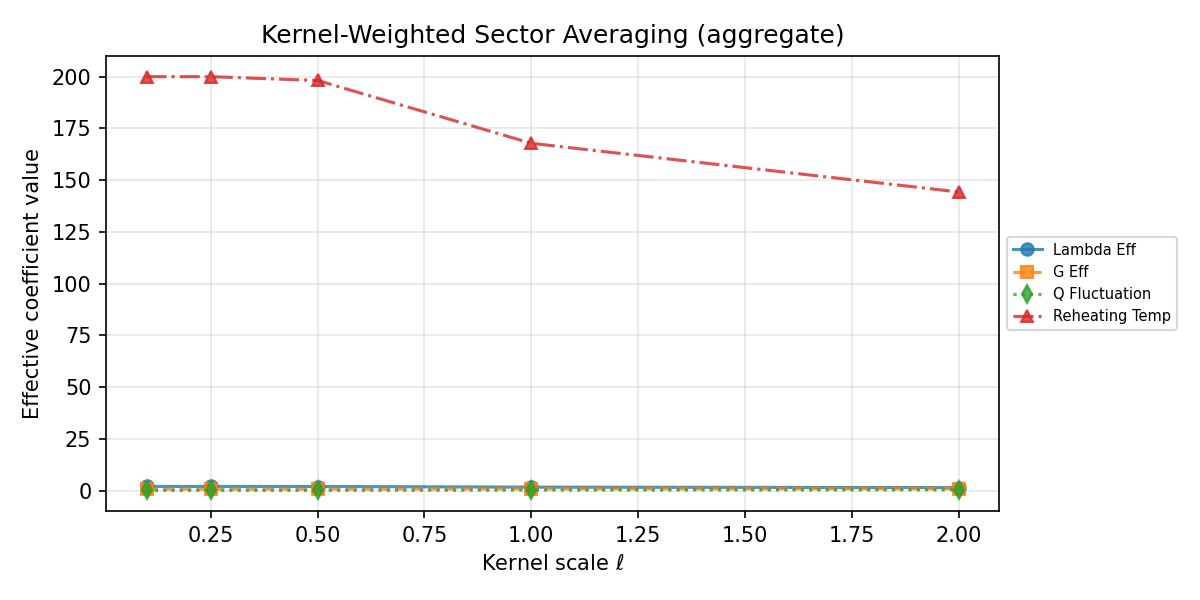
\includegraphics[width=\columnwidth]{figures/fig_06_effective_coefficient_flow.png}
  \caption{Kernel-weighted sector averaging under unobserved-sector mixing.
  As $\ell$ increases, aggregate parameters interpolate between the
  $x_0$ basin values and the global average.}
  \label{fig:coeff_flow}
\end{figure}

\subsection{Full ell sensitivity table}
\label{app:ell_sensitivity_full}

\begin{table*}[t]
  \centering
  \caption{Ell sensitivity: ISR (Gaussian kernel) stability metrics across kernel scale $\ell$ (non-degenerate regime, $\ell \ge 0.48$). The physically meaningful regime begins at $\ell \approx 0.5$, where $N_{\rm eff}$ exceeds $\sim 30\%$ of $N$. Small-$\ell$ and boundary values are diagnostic artifacts reported in Appendix~\ref{app:degenerate}. The baseline global-census KL is $3.58\times10^{-4}$.}
  \label{tab:ell_sensitivity}
  \small
  \begin{tabular}{lcccccc}
    \toprule
    $\ell$ & $N_{\rm eff}$ & KL drift & Wasserstein & Basin exc. rate & $\Lambda_{\rm eff}$ & Conv. rate \\
    \midrule
    0.48 & 3629 & $1.8\times10^{-6}$ & $2.4\times10^{-4}$ & 0.00 & 1.986 & $-1.22$ \\
    0.71 & 4793 & $4.3\times10^{-5}$ & $2.9\times10^{-3}$ & 0.00 & 1.868 & $-1.07$ \\
    1.00 & 7176 & $1.3\times10^{-4}$ & $6.6\times10^{-3}$ & 0.01 & 1.662 & $-0.93$ \\
    1.51 & 8841 & $1.9\times10^{-4}$ & $8.1\times10^{-3}$ & 0.27 & 1.511 & $-0.87$ \\
    2.20 & 9563 & $2.3\times10^{-4}$ & $8.6\times10^{-3}$ & 0.59 & 1.427 & $-0.91$ \\
    3.21 & 9860 & $2.7\times10^{-4}$ & $8.9\times10^{-3}$ & 0.61 & 1.384 & $-0.95$ \\
    10.00 & 9998 & $3.4\times10^{-4}$ & $9.2\times10^{-3}$ & 0.67 & 1.347 & $-0.98$ \\
    \bottomrule
  \end{tabular}
\end{table*}


\begin{figure}[t]
  \centering
  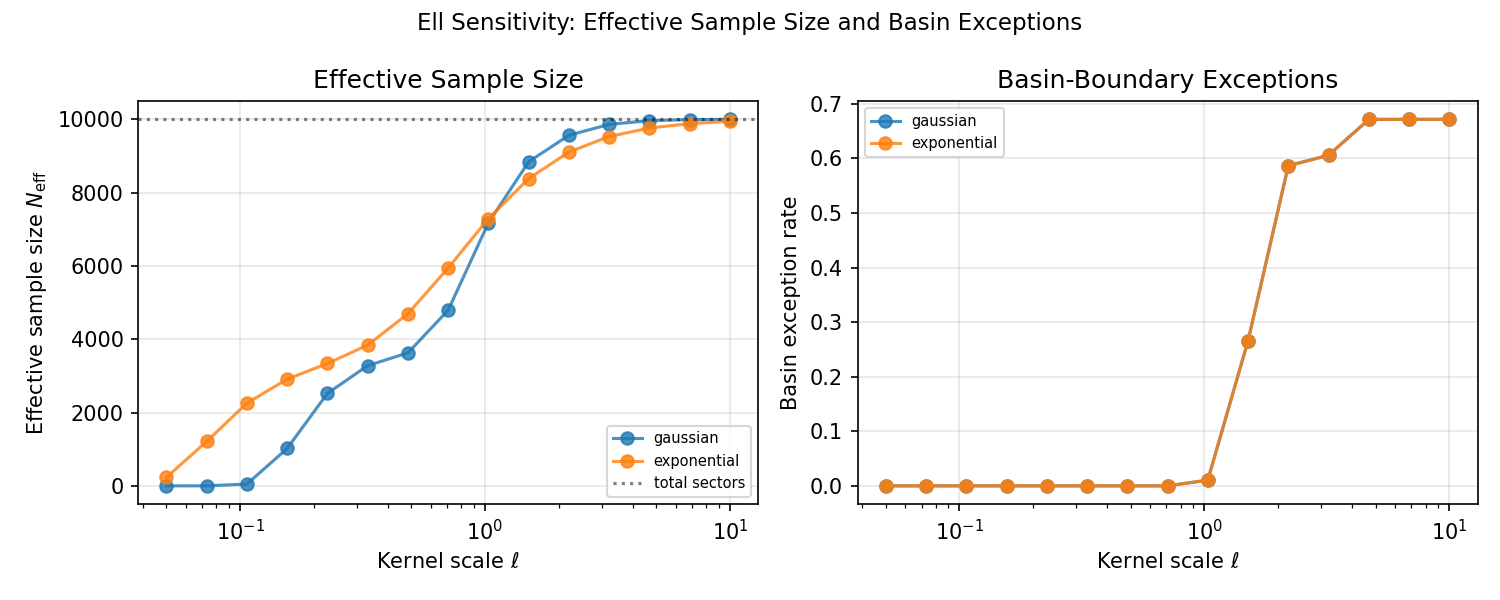
\includegraphics[width=\columnwidth]{figures/fig_12_ell_sensitivity_neff.png}
  \caption{Effective sample size $N_{\rm eff}$ and basin exception rate
  vs.\ $\ell$. The sweet spot lies where $N_{\rm eff}$ is large enough
  for statistical power but basin exceptions remain below 30\%.}
  \label{fig:ell_sensitivity_neff}
\end{figure}

\subsection{Degenerate small-$\ell$ behavior}
\label{app:degenerate}

When the kernel scale $\ell$ is much smaller than the inter-vacuum spacing
($\ell \lesssim 0.25$), the Gaussian kernel assigns non-negligible weight only
to sectors in the $x_0$ basin.
The effective sample size drops to $N_{\rm eff} \ll N$, and the ISR
distribution is effectively a delta function on the $x_0$ vacuum.
KL divergence between successive cutoffs vanishes trivially
($<10^{-25}$ at $\ell=0.05$) because there is no distribution to shift.

These values are reported separately here because they are diagnostic
artifacts, not evidence of physical stability.
Including them alongside non-degenerate results would misleadingly inflate
the apparent improvement ratio.

Tables~\ref{tab:degenerate_ell_sensitivity}~and~\ref{tab:degenerate_sigma_ell}
show the degenerate and boundary rows.

\begin{table*}[htbp!]
  \centering
  \caption{Degenerate and boundary rows from the ell sensitivity scan
  (Gaussian kernel). Rows with $\ell \lesssim 0.25$ are degenerate:
  $N_{\rm eff} \ll N$, producing trivially vanishing KL drift.
  The $\ell = 0.23$ row ($N_{\rm eff}/N = 0.25$) is a boundary case
  that narrowly fails the $N_{\rm eff}/N \ge 0.3$ threshold.}
  \label{tab:degenerate_ell_sensitivity}
  \small
  \begin{tabular}{lcccccc}
    \toprule
    $\ell$ & $N_{\rm eff}$ & KL drift & Wasserstein & Basin exc. rate & $\Lambda_{\rm eff}$ & Conv. rate \\
    \midrule
    0.05 & 1.0 & $<10^{-25}$ & $<10^{-125}$ & 0.00 & 2.000 & --- \\
    0.10 & 49.6 & $<10^{-29}$ & $<10^{-29}$ & 0.00 & 2.000 & --- \\
    0.23 & 2523 & $2.0\times10^{-10}$ & $1.6\times10^{-9}$ & 0.00 & 2.000 & $-0.07$ \\
    \bottomrule
  \end{tabular}
\end{table*}

\begin{table*}[htbp!]
  \centering
  \caption{Full sigma--ell boundary grid including degenerate small-$\ell$
  columns. Values at $\ell=0.10$ and $\ell=0.25$ are diagnostic artifacts:
  the narrow kernel forces $N_{\rm eff} \ll N$, producing trivially large
  improvement ratios.}
  \label{tab:degenerate_sigma_ell}
  \small
  \begin{tabular}{lccccc}
    \toprule
    $\sigma$ $\backslash$ $\ell$ & 0.10 & 0.25 & 0.50 & 1.00 & 2.00 \\
    \midrule
    0.5 & $2.0\times10^{21}$ & $5.6\times10^{6}$ & 68.5 & 3.12 & 1.28 \\
    1.0 & $9.6\times10^{20}$ & $2.9\times10^{5}$ & 142.5 & 5.97 & 1.86 \\
    1.5 & $1.1\times10^{21}$ & $4.1\times10^{5}$ & 240.0 & 5.38 & 2.35 \\
    2.0 & $9.2\times10^{20}$ & $2.1\times10^{5}$ & 103.1 & 7.68 & 4.40 \\
    3.0 & --- & $9.5\times10^{5}$ & 58.5 & 6.27 & 2.46 \\
    \bottomrule
  \end{tabular}
\end{table*}


\end{document}
